\documentclass[journal,10pt,onecolumn,compsoc]{IEEEtran} \usepackage[margin=1.0in]{geometry} \usepackage{pdfpages} \usepackage{graphicx} 
\graphicspath{/graphics} \setlength{\parskip}{\baselineskip} \setlength\parindent{24pt}
\usepackage[english]{babel}
%\usepackage{fullpage}

\newcommand*\Title{Requirements Document for VisualFlow}
\newcommand*\Date{November 2016}
\newcommand*\Author{Connor Sedwick, Behnam Saeedi, Collin Dorsett}
\newcommand*\GroupNumber{Group Number: 33}
\newcommand*\GroupName{Group Name: Visual Flow}
\title{Requirements Document for VisualFlow}
\author{Connor Sedwick, Behnam Saeedi,  Collin Dorsett}
\date{\today}

\begin{document}
\maketitle
\noindent \textbf{Abstract} \\
			\indent 
			Software that allows individuals to visualize the step-by-step process of computer programming has greatly assisted aspiring programmers and experienced professionals.
	In the professional world, visualization software allows people in industry a tool to analyze data and develop a more concrete understanding of the architecture of a system. 
	Tools that aid individuals in programming software exist for both educational and commercial purposes, but there is a lack of visualization software targeted specifically at the subject of machine learning.
			TensorFlow is a machine learning API (Application Program Interface) developed by Google in order to provide an optimized machine learning toolset for developers.
			 This toolset is designed to be an all-in-one machine learning solution for users who do not have the time, technical skills or resources to produce their own methods.
			 Despite TensorFlow having useful applications and a rich manual it does not have an eloquent way to interact with visualization of the software for its users.
			 To address this issue we wish to develop a product that can display data between nodes in a computational graph and designing a network would be as easy as placing nodes and drawing connections between them.
			 This solution will take advantage of simple shapes to abstract basic programming concepts.
			 This system will represent the complex program as simple flowchart like diagrams to the user.
%			 Another important aspect of our system is Runtime Tuning.
%			 Runtime Tuning is manipulation of data and variables during the runtime of a program in order to help users in improving the performance of their solution.
%			 Our proposed Graphical User Interface (GUI) will offer sets of features in order to make this task easier.
%			 Our target audience is individuals with little to no experience with machine learning or computer programming who specialize in fields such as statistics, data analysis and mathematics.\\

\newpage
\tableofcontents
\newpage
\section{Introduction}

This section gives a scope description and overview of everything included in this SRS document. 
The purpose for this document is described here and a list of abbreviations and definitions is provided within this section.

\subsection{Purpose}

The purpose of this document is to give a detailed description of the requirements for the WYSIWYG Deep Learning graphical user interface software. It will illustrate the purpose and complete declaration for the development of the system. 
It will also explain system constraints, interface and interactions with other external applications. 

\subsection{Scope}

The WYSIWYG Deep Learning graphical user interface is an application which helps users design and test deep learning algorithms.
This tool will be developed to comply with Google's Deep learning API called "TensorFlow\texttrademark".
This solution allows developers to use their implementation alongside their data in order create their deep learning applications.

\subsection{Glossary}
\begin{itemize}
	\item \textbf{WYSIWYG:}
		This is an abbreviation for "What You See Is What You Get".
		Microsoft PowerPoint and LibreOffice Impress are two good examples of such system. 
		In this system, the end result is very similar to user's preview of the output during the development.\\
	\item \textbf{Tensorflow\texttrademark:}
		TensorFlow\texttrademark is an open source software library for numerical computation using data flow graphs.
		TensorFlow\texttrademark was originally developed by researchers and engineers working on the Google Brain Team within Google's Machine Intelligence research organization for the purposes of 
		conducting machine learning and deep neural networks research, but the system is general enough to be applicable in a wide variety of other domains as well.\\
	\item \textbf{GUI:}
		GUI or Graphical User Interface, is an interface that allows users to interact with a given system through graphical icons as opposed to a text based, command-line representation.\\
	\item \textbf{Scene:}
		The work space where user can place different elements of their program.\\
	\item \textbf{Block:}
		A block is a GUI feature that represents a data structure or line of code. A block could be a variable, a constant, a method, a class, a probe, input or output.\\
	\item \textbf{Block-Menu:}
		A menu that contains all of the items and functionality icons that are ready to be dragged and dropped into the scene.\\
	\item \textbf{Run:}
		The task of starting the execution of a program.\\
	\item \textbf{Stop:}
		Brings the execution of the program to a halt. Resuming the process requires running the program again.
		This functionality will reset the state of the execution.\\
	\item \textbf{Extract:}
		A command that allows the user to pull the current version of their solution and save the file in a user-chosen space in memory.
		In order for a user to have a stand-alone version of their implemented program, they need to extract their project.\\
	\item \textbf{Variable/Constant:}
		Variables are equivalent to programming variables. They are represented by rhombuses in our graphical user interface.
		Constants are similar to  variables, however, these values can not be changed while running the program.
		Constants are also represented by rhombuses.\\
	\item \textbf{Method:}
		A function from the API that perform a specific task. They are represented by boxes.
		The circles on the edges of a method box are inputs and outputs of that method.\\
	\item \textbf{Class:} 
		An object that contains multiple variables and methods (public or private).
		Classes are represented as transparent boxes around methods and variables. This box could be abstracted away to be displayed as a solid color box.\\
	\item \textbf{Abstract:}
		A feature of a class that will turn the class from transparent to solid color in order to hide the content of the class.\\
	\item \textbf{Layer:} 
		An instance of a Scene. 
		These instances could be independently implemented so that they function individually.
		Layers can be run individually and they will generate data from input.\\
	\item \textbf{Channel:}
		 A connection between inputs and outputs that display the direction of data flow and route the data from one Block to another.\\
	\item \textbf{Probe:}
		A Block type that displays the content of a channel.
		Can modify the value which is being transmitted through the Channel it is placed on.
		If the value of a Probe is modified, the modification will happen after the point which the probe is inserted into the Channel.
		Every value that goes though the Channel before the probe is left unchanged with the exception of pointer Probes.\\
	\item \textbf{Input:}
		A Block type which allows the user to insert data into their program during the run process.\\
	\item \textbf{Output:}
		A Block type which allows the user to see the final result. Outputs indicate discontinuation of a Channel.\\
\end{itemize}
\subsection{References}
References

[1]"WYSIWYG - definition of WYSIWYG in English | Oxford Dictionaries", Oxford Dictionaries | English, 2016. [Online]. Available: https://en.oxforddictionaries.com/definition/WYSIWYG. [Accessed: 03- Nov- 2016].\\

[2]"What is graphical user interface (GUI)? definition and meaning", BusinessDictionary.com, 2016. [Online]. Available: http://www.businessdictionary.com/definition/graphical-user-interface-GUI.html. [Accessed: 03- Nov- 2016].\\

[3]"Cite a Website - Cite This For Me", Tensorflow.org, 2016. [Online]. Available: https://www.tensorflow.org/. [Accessed: 03- Nov- 2016]. \\
%\begin{thebibliography}{7}
%	\bibitem{latexcompanion} 
%	potato face 1, potato face 2, potato face 3. 
%	\textit{The \LaTeX\ Companion}. 
%	Addison-Wesley, Reading, Massachusetts, 1993.
 
%	\bibitem{einstein} 
%	Albert Einstein. 
%	\textit{Zur Elektrodynamik bewegter K{\"o}rper}. (German) 
%	[\textit{On the electrodynamics of moving bodies}]. 
%	Annalen der Physik, 322(10):891–921, 1905.
 
%	\bibitem{knuthwebsite} 
%	Knuth: Computers and Typesetting,
%	\\\texttt{http://www-cs-faculty.stanford.edu/\~{}uno/abcde.html}
%\end{thebibliography}

\subsection{Overview}

The following sections provide an overview of the system functionality and system interaction with other libraries and user custom functions. 
Chapter two introduces different types of users and their interaction with the system. 
Furthermore, it also mentions the system constraints and assumptions.

\noindent The third chapter provides the requirement specifications in detailed terms and a description of the different system interfaces. 
Different specification techniques are used in order to specify the requirements more precisely for different audiences.

\newpage

\section{Overall Description}

This section will give an overview of the TensorFlow\texttrademark WYSIWYG system. 
The software will be explained in its context to show how the software interfaces with external libraries and introduce the basic functionality of it. 
It will also describe types of users  and functionalities that are available for each type of user based on their needs. 
By the end, the constraints and assumptions for the system will be presented.

\subsection{Product Perspective}

This software will consist primarily of the graphical user interface which will communicate with Google's TensorFlow\texttrademark library. 
This software requires access to the TensorFlow\texttrademark library for the duration of development, execution and extraction. 
The interface will provide basic design and flow of data through user's program in a flowchart-like visual representation (WYSIWYG).
The underlying code and algorithm designed by the user will be assembled in a file which is built and saved in the background. 

\subsection{Product Functions}

With WYSIWYG graphical user interface, users will be able to design an algorithm by placing and connecting uniquely shaped blocks in a build space.
Furthermore, in the WYSIWYG GUI, drawing connections between the Blocks represents dependencies, calls and flow of the data in the system.
Build spaces represent files, classes or layers that are required to perform user's designated task.
Files will be built based on the Blocks and connections drawn between them in a build space.
These files can be extracted and saved to a user-designated folder at the push of a button.
The extracted files are human readable and in the base language of Google's TensorFlow\texttrademark API (Python).

\noindent Developers will be able to set Probes on connections drawn between Blocks to either modify values or track values as they are manipulated by their algorithm.
Helpful Python compliant errors, warnings and alerts will let the user know if there is an error with the way they have designed their algorithm or execution errors with their custom Blocks.

\subsection{User Characteristics}

There are many types of users who will likely use this software. 
The target users of this tool includes but is not limited to people who need to practice high level programming solutions such as machine learning techniques and lack the technical skills that are required to implement them.
As it stands, there is only one development layout to be used for the graphical user interface.
All users will be using the same interface whether they are students, developers, or employees whose project relies on deep learning software. 
However, WYSIWYG solution does support custom Blocks for users who are capable of implementing their own functions.

\subsection{Constraints}

This project is very user based and constraints are only imposed on usability of our software and the core library that we are trying to mask. 
This naturally prohibits users from modifying and tampering with the code provided by Google's TensorFlow\texttrademark API since it forces the tool set to recreate all the GUI elements.
The graphical user interface must be easily understood by the user and developer.
The display of results must be reliable and dependable.
The core system has its own limitations which will limit our GUI.

\subsection{Assumptions and Dependencies}

One assumption we have is that not all users will have prior knowledge on software programming when using this software.
A user may not know what a variable is or what a function is and how it relies on variables. 
When piecing together an algorithm a user may not know the proper syntax that would be required when using a text editing software.

\noindent A dependency for this software is access to Google's TensorFlow\texttrademark library from the user's memory space. 
This will require a user to install the the software along with TensorFlow\texttrademark otherwise the software will not be usable in some scenarios.

\subsection{Apportioning of Requirements}

In the case that the project is delayed, there are some requirements that could be transferred to the next version of the application. 
This flexibility allows user to use features that are already available without worrying about how new features might affect their system.

\begin{minipage}{\textwidth}
		\fbox{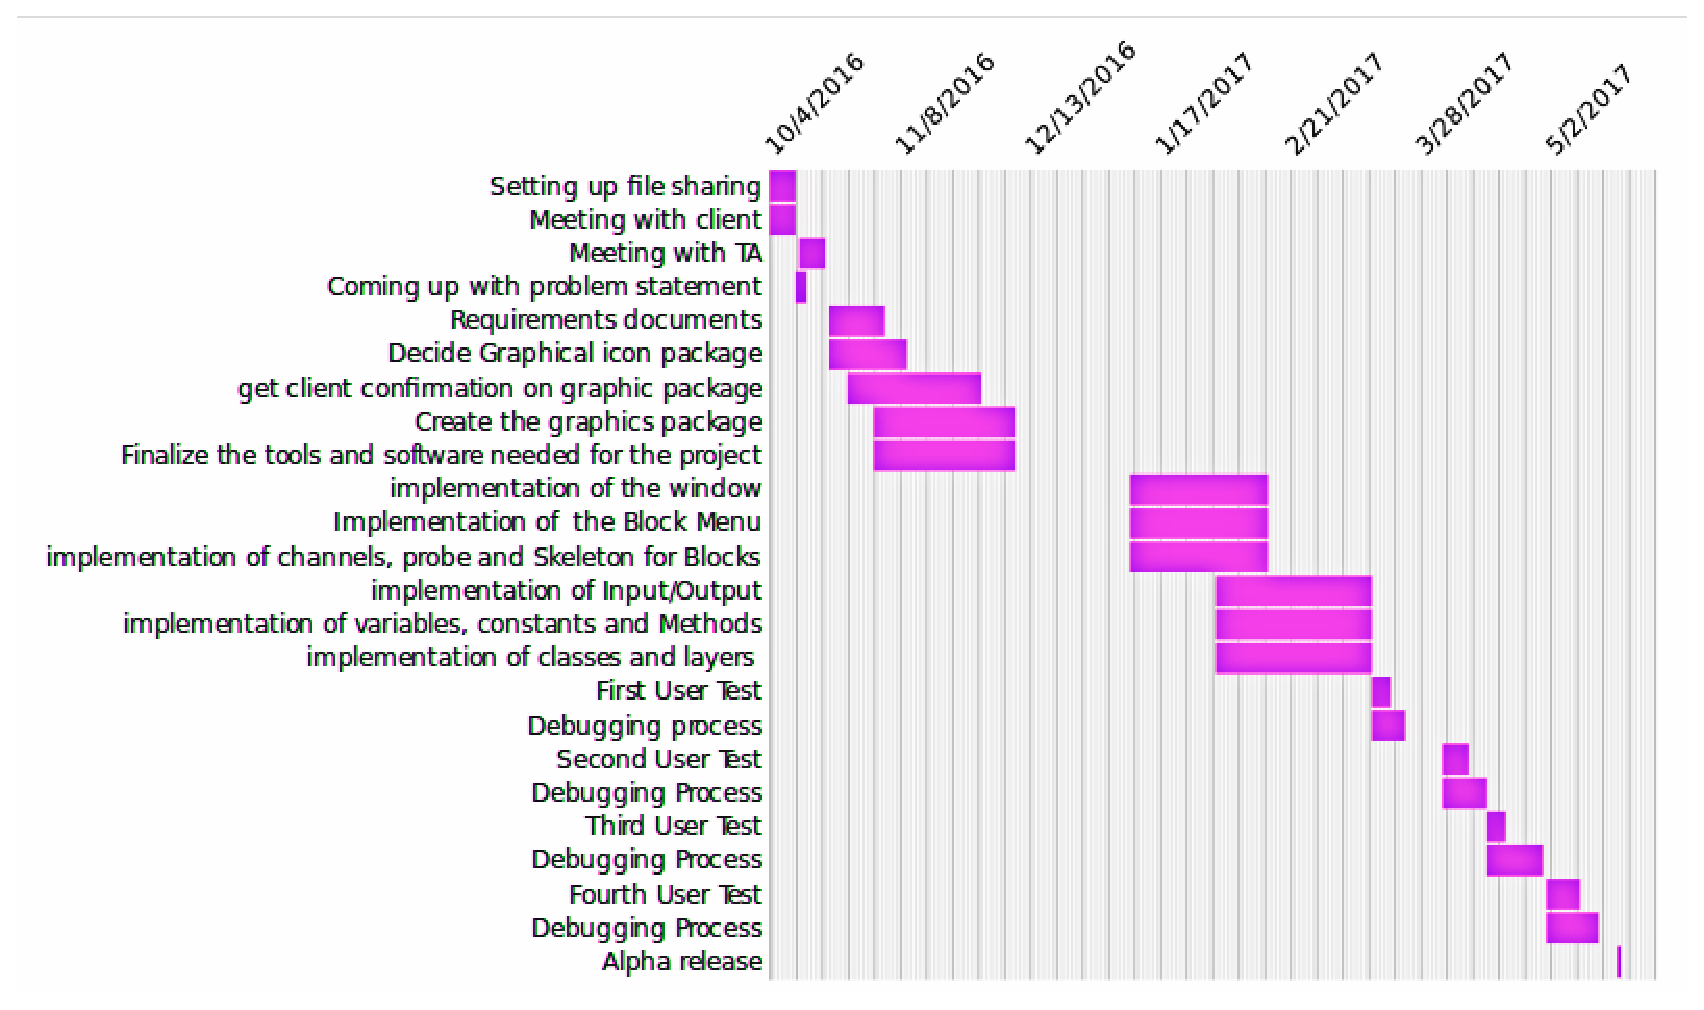
\includegraphics[width=1.0\textwidth]{graphics/Gantt-Chart.eps}}\\
%		\label{fig:fig1}
%		\caption{A proposed layout of the menu and build space.}
	\end{minipage}


\newpage

\section{Specific Requirements}

This section contains all of the functional and quality requirements of this solution to the WYSIWYG system. 
It provides a detailed description of the system and all its core features.


\subsection{Interfaces}
\subsubsection{User Interfaces}

The graphical user interface will begin by displaying a menu allowing the user to "Start a new project."
Once this is chosen, "Scene" is created and the user will be brought to the main menu screen and build space.
From this screen the user will have the ability to choose different types of Blocks for either coding or debugging purposes.
There will be buttons that allow users to build their file and Run it.

\noindent User has the ability to "Import" or "Export" code.
This feature allows user to turn their code into a block to use with WYSIWYG GUI or export their system into code.
This will be done by pressing a button and choosing a place in memory to load or store the code. 
The file should be loaded from or stored in a file with a ".py" extension.

\subsubsection{Software Interfaces}

The graphical user interface masks away the core of the solution. Its job is to systematically assemble the Python code as text interpreted from the flowchart.
Furthermore, the GUI directly interacts with the pre-installed Python server on the operating system.
If an error message is thrown the interface should catch and display the error to the user as a formatted message within the GUI.
This message is generated by the Python interpreter.

\subsection{Functional Requirements}

This section includes the requirements that specify the fundamental actions of the software system.
Furthermore, it describes the necessary outcomes that are expected by the client.

\noindent
\textbf{ID: FR1}\\
TITLE: Download the application\\
DESC: A user should be able to download the software from an application store, GitHub or some online repository. 
The software should support TensorFlow\texttrademark's pre-implemented methods from their library. \\
RAT: In order for the user to download the software and have access to the required libraries.\\
DEPEND: None\\

\noindent
\textbf{ID: FR2}\\
TITLE: Open the GUI and start session\\
DESC: A user should be able to start a new session. \\
RAT: In order for the user to open up and start a new project with a blank build space.\\
DEPEND: FR1\\

\noindent
\textbf{ID: FR3}\\
TITLE: Session/Project Directory\\
DESC: The software should create a directory with a name specified by the user upon starting a new session or project.
This task is handed to the operating system. This means the permissions for the folders depend on user that uses the GUI. \\
RAT: In order for the software to build and store user files related to the current project in a main directory.\\
DEPEND: FR2\\

\noindent
\textbf{ID: FR4}\\
TITLE: Block-Menu\\
DESC: The software should contain a Block menu.\\
RAT: In order for the user to find Blocks for the building of their algorithm.\\
DEPEND: FR2\\

\noindent
\textbf{ID: FR5}\\
TITLE: Build Space / Scene\\
DESC: The software should offer a blank space box within the GUI for users to place Blocks.\\
RAT: In order for the user to find Blocks for the building of their algorithm.\\
DEPEND: FR2\\

\noindent
\textbf{ID: FR6}\\
TITLE: Drag and drop\\
DESC: The software should allow the user to drag Blocks from the Block Menu and place them in a build space.\\
RAT: In order for the user to manipulate their algorithm.\\
DEPEND: FR3\\

\noindent
\textbf{ID: FR7}\\
TITLE: Channel drawing\\
DESC: The software should allow users to draw a Channel between two Blocks. 
This should be done simply by selecting them by clicking on them and choosing an option to "Draw channel".\\
RAT: In order for the user to send values between Blocks.\\
DEPEND: FR3, FR4\\

\noindent
\textbf{ID: FR8}\\
TITLE: Blocks manipulation\\
DESC: The software should allow users to enter numerical and string values into variable Blocks and Probes.\\
RAT: In order for the user to write their algorithm.\\
DEPEND: FR4\\

\noindent
\textbf{ID: FR9}\\
TITLE: Background file creation\\
DESC: The software should create and update user files every time user choses to save their scene. 
Files should be updated in a user-defined directory.\\
RAT: In order for the user to have a raw and formatted file of their software.\\
DEPEND: FR2, FR3, FR6, FR7, FR8\\

\noindent
\textbf{ID: FR10}\\
TITLE: Build button\\
DESC: The software should create all files in the user's build directory at a single press of the Build button. 
A Python-compatible file should appear in the user's current project directory if the implementation is Python-compliant.\\
RAT: In order for the user to create a Python-compliant file in order to run the software.\\
DEPEND: FR4\\

\noindent
\textbf{ID: FR11}\\
TITLE: Error handling\\
DESC: The software should display a text box or error message to the screen letting the user know if there is an error with their build. 
There should also be a helpful hint on what the user may do to fix their problem if the issue is caused by misuse of the GUI.\\
RAT: In order for the user to know that there is an issue with the formatting of the current build of their software implementation.\\
DEPEND: FR10\\

\noindent
\textbf{ID: FR12}\\
TITLE: Data input\\
DESC: The software should allow the user to include a file of their own data to be used by their software.
This feature is defined by the input feature.\\
RAT: In order for the user to test their software on their own data.\\
DEPEND: FR2\\

\noindent
\textbf{ID: FR13}\\
TITLE: Layered builds\\
DESC: A user should be able to create multiple layers to their software by opening multiple build spaces.\\
RAT: In order for the user to visualize the structure of their software.\\
DEPEND: FR2\\

\noindent
\textbf{ID: FR14}\\
TITLE: File extraction\\
DESC: The software should allow the user to save their current build file to a user-chosen space in memory.\\
RAT: In order for the user to have a raw and formatted file of their software in designated storage.\\
DEPEND: FR4\\


\subsection{Performance Requirements}

The requirements in this section provide a detailed specification of the user interaction with the software and measurements placed on the system's performance.

\noindent
\textbf{ID: QR1}\\
TITLE: Easy installation\\
DESC: There should be a simple downloadable package including everything required to begin using the software after installation.
There should be a different installation package depending on the operating system being used.\\
RAT: In order for the user to being using the software without having to worry about file dependencies.\\
DEPEND: None\\

\noindent
\textbf{ID: QR2}\\
TITLE: Prominent Block Menu\\
DESC: The Block Menu for the flowchart pieces should contain labelled Blocks and be legible.\\
RAT: In order for the user to navigate the menu and find specific Block types easily.\\
DEPEND: None\\

\noindent
\textbf{ID: QR3}\\
TITLE: Prominent feature buttons\\
DESC: The buttons used to build and run the software should be easy to distinguish between each other. 
For example, the extraction button should be indicated by as a button labelled "Extract".
Buttons should respond to a single click and respond within less than a second of the user clicking them.\\
RAT: In order to avoid confusion when trying to build and run the program.\\
DEPEND: None\\

\noindent
\textbf{ID: QR4}\\
TITLE: Prominent alerts\\
DESC: Alerts signaled by the compiler should be displayed to the screen as soon as they are sent. 
When an error has been fixed its corresponding alert should disappear.
Alerts should appear in colored text boxes: red boxes for fatal errors, yellow boxes for warnings.\\
RAT: This will cut down on confusion when rebuilding a file and trying to find issues with a solution.\\
DEPEND: None\\

\noindent
\textbf{ID: QR5}\\
TAG: Response time\\
DESC: The speed at which the interface communicates with the TensorFlow\texttrademark library and displays output to the screen.\\
SCALE: The time of a build.\\
METER: Measurements obtained by 1000 builds during testing.\\
MUST: No more than 3 seconds 100\% of the time.\\
WISH: No more than 2 seconds 100\% of the time.\\

%\subsection{Design Requirements}
%\subsection{Software System Attributes}
%\newpage


%\newpage
%\section{References}
%\newpage

%\section{Gantt}
%\begin{figure}
%	\begin{minipage}{\textwidth}
%		\fbox{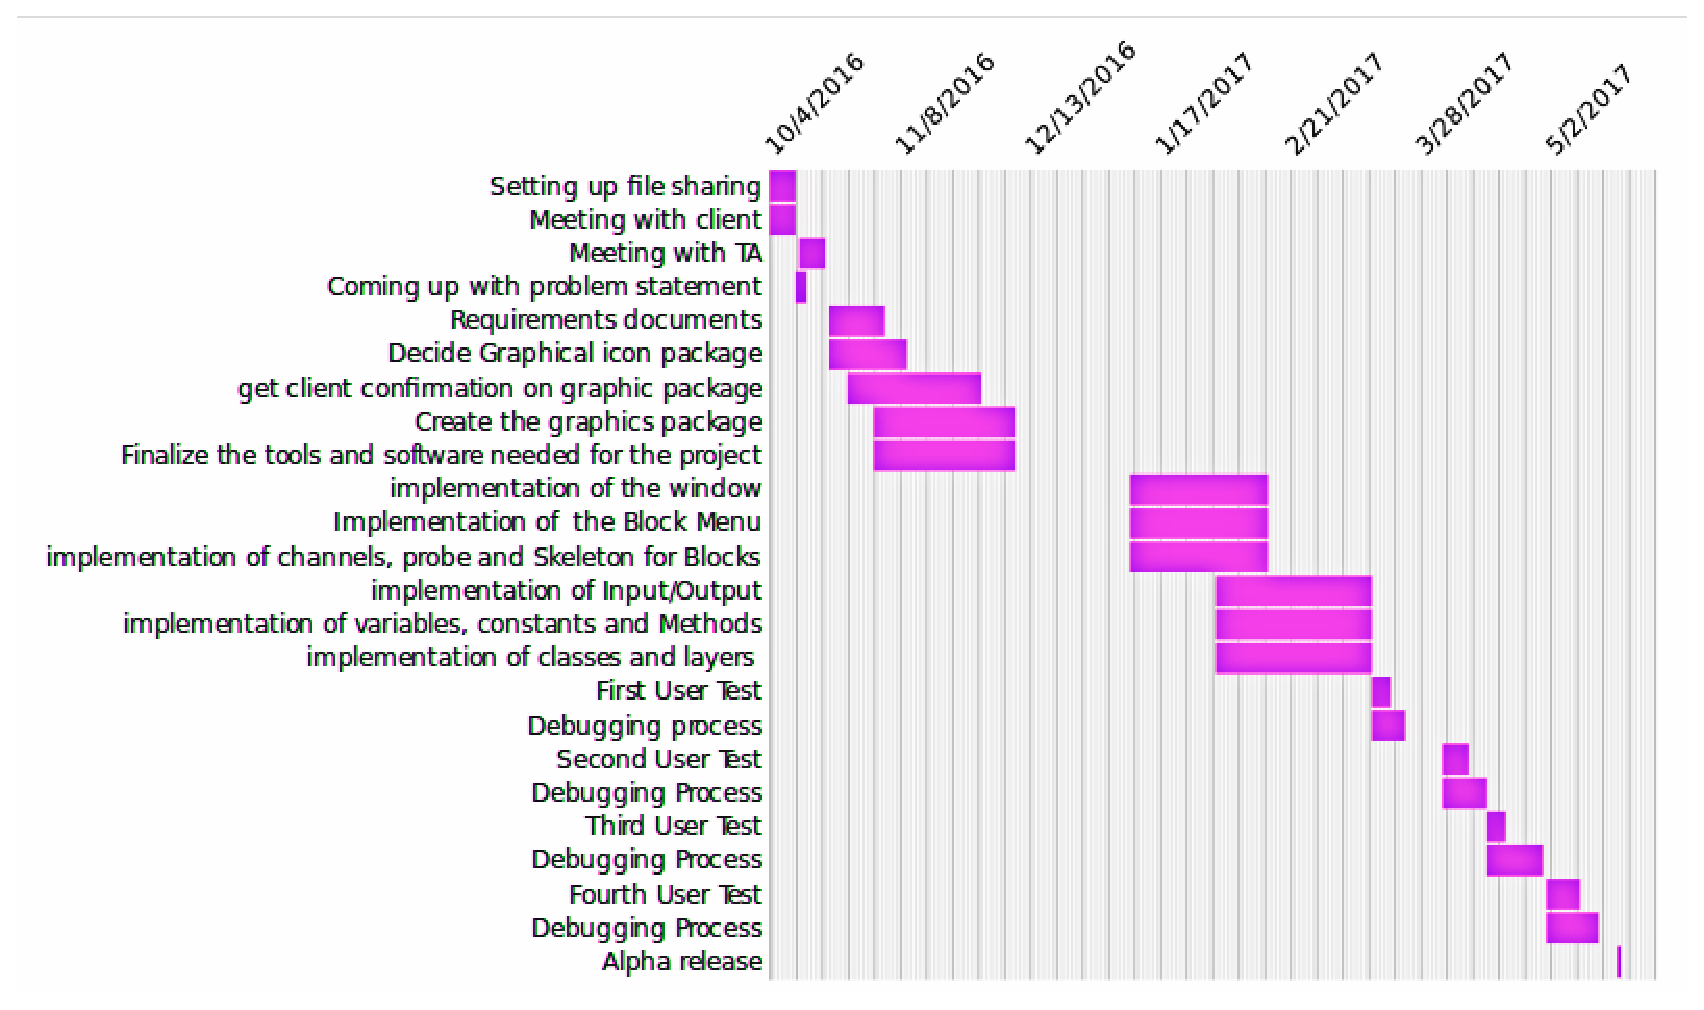
\includegraphics[width=1.0\textwidth]{graphics/Gantt-Chart.eps}}\\
%		\label{fig:fig1}
%		\caption{A proposed layout of the menu and build space.}
%	\end{minipage}
%	\end{figure}

\end{document}
